%% Source of figures/smote-dp-equations.pdf (six pages, one per decision point).
%% Compile: pdflatex smote-dp-equations.tex
%% Figures 2 to 7 of the Method part draft (Claude, 29 Oct 2026): each decision point as an
%% equation that extends the SMOTE rule, with SMOTE's own choice, the general form (changed
%% part in colour), an example from a method in the corpus, and a sketch on 2-D data.
\documentclass[tikz,border=4pt]{standalone}
\usepackage[scaled]{helvet}\renewcommand{\familydefault}{\sfdefault}
\usepackage{amsmath,amssymb,bm}
\usetikzlibrary{arrows.meta,positioning,calc,shapes.geometric,backgrounds,decorations.pathreplacing}
\definecolor{cSeed}{HTML}{2A78D6}\definecolor{cAlloc}{HTML}{EB6834}\definecolor{cNbr}{HTML}{1BAF7A}
\definecolor{cPlace}{HTML}{C98A00}\definecolor{cFilt}{HTML}{C0392B}\definecolor{cPipe}{HTML}{7B4FA0}
\definecolor{inkTwo}{HTML}{465462}\definecolor{maj}{HTML}{A3ABB4}\definecolor{minc}{HTML}{8DB6E8}
\newcommand{\x}{\mathbf{x}}
\tikzset{
  ttl/.style={anchor=north west,font=\bfseries\large,text=#1},
  hd/.style={anchor=north west,font=\scriptsize\bfseries,text=inkTwo},
  eq/.style={anchor=north west,align=left,text width=9.6cm,font=\normalsize},
  note/.style={anchor=north west,align=left,text width=9.6cm,font=\scriptsize,text=inkTwo},
  mn/.style={circle,fill=minc,minimum size=6.5pt,inner sep=0pt},
  mj/.style={rectangle,fill=maj,minimum size=6pt,inner sep=0pt},
  sy/.style={star,star points=5,fill=#1,minimum size=8pt,inner sep=0pt},
  panel/.style={draw=inkTwo!40,rounded corners=4pt},
}
% common left column: title, SMOTE line, general line, example line
\newcommand{\ind}{\mathbf{1}}
\newcommand{\leftcol}[6]{%
  \node[ttl=#1,inner sep=0pt] (T) at (0,0) {#2};
  \node[hd,inner sep=0pt] (H1) at ($(T.south west)+(0,-0.3)$) {SMOTE (2002)};
  \node[eq,text=inkTwo,inner sep=0pt] (E1) at ($(H1.south west)+(0,-0.12)$) {#3};
  \node[hd,inner sep=0pt] (H2) at ($(E1.south west)+(0,-0.3)$) {Generalised};
  \node[eq,inner sep=0pt] (E2) at ($(H2.south west)+(0,-0.12)$) {#4};
  \node[hd,inner sep=0pt] (H3) at ($(E2.south west)+(0,-0.3)$) {Example in the corpus};
  \node[eq,font=\small,inner sep=0pt] (E3) at ($(H3.south west)+(0,-0.12)$) {#5};
  \node[note,inner sep=0pt] (N) at ($(E3.south west)+(0,-0.25)$) {#6};
}
\begin{document}

%% ---------------- 1. seed selection ----------------
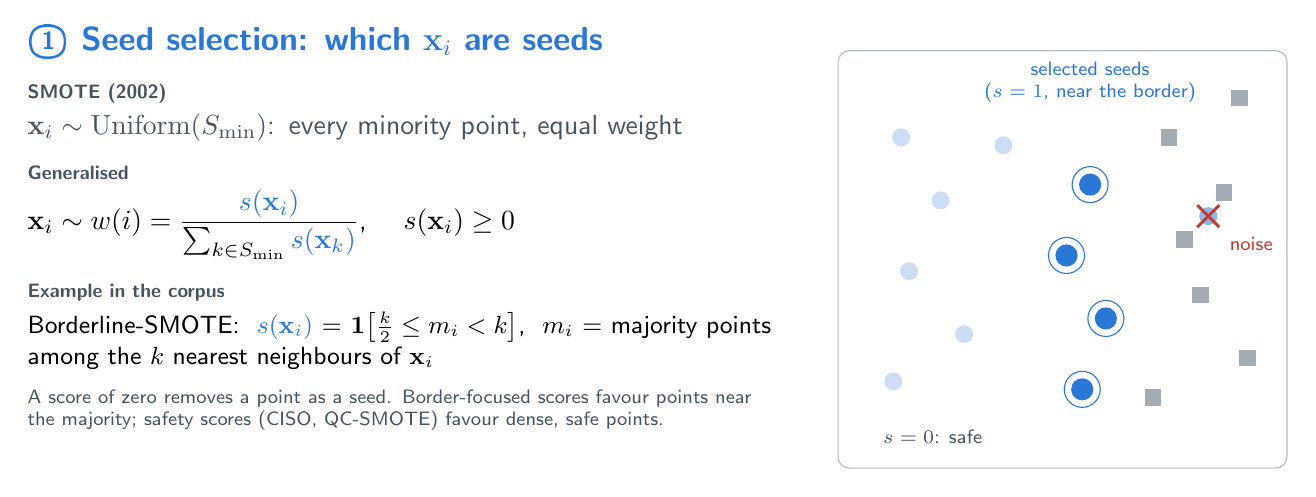
\begin{tikzpicture}
\leftcol{cSeed}{\textcircled{\small 1} Seed selection: which $\x_i$ are seeds}
 {$\x_i \sim \mathrm{Uniform}(S_{\min})$: every minority point, equal weight}
 {$\x_i \sim w(i) = \dfrac{\textcolor{cSeed}{s(\x_i)}}{\sum_{k\in S_{\min}} \textcolor{cSeed}{s(\x_k)}}$, \quad $s(\x_i)\ge 0$}
 {Borderline-SMOTE: \ $\textcolor{cSeed}{s(\x_i)} = \ind\!\left[\tfrac{k}{2}\le m_i < k\right]$, \ $m_i$ = majority points among the $k$ nearest neighbours of $\x_i$}
 {A score of zero removes a point as a seed. Border-focused scores favour points near the majority; safety scores (CISO, QC-SMOTE) favour dense, safe points.}
\begin{scope}[shift={(10.6,-5.3)}]
\draw[panel] (-0.3,-0.3) rectangle (5.4,5.0);
\foreach \p in {(3.9,3.9),(4.6,3.2),(4.3,1.9),(4.9,1.1),(3.7,0.6),(4.8,4.4),(4.1,2.6)} \node[mj] at \p {};
\foreach \p in {(0.5,3.9),(1.0,3.1),(0.6,2.2),(1.3,1.4),(0.4,0.8),(1.8,3.8)} \node[mn,opacity=0.45] at \p {};
\foreach \p in {(2.9,3.3),(3.1,1.6),(2.6,2.4),(2.8,0.7)} {\node[circle,fill=cSeed,minimum size=8pt,inner sep=0pt] at \p {}; \node[circle,draw=cSeed,minimum size=13pt,inner sep=0pt] at \p {};}
\node[mn] (nz) at (4.4,2.9) {};
\draw[cFilt,line width=1pt] ($(nz)+(-0.14,-0.14)$)--($(nz)+(0.14,0.14)$) ($(nz)+(-0.14,0.14)$)--($(nz)+(0.14,-0.14)$);
\node[font=\scriptsize,text=cSeed,align=center] at (2.9,4.6) {selected seeds\\ ($s=1$, near the border)};
\node[font=\scriptsize,text=inkTwo] at (0.9,0.1) {$s=0$: safe};
\node[font=\scriptsize,text=cFilt,anchor=west] at (4.55,2.55) {noise};
\end{scope}
\end{tikzpicture}

%% ---------------- 2. sample allocation ----------------
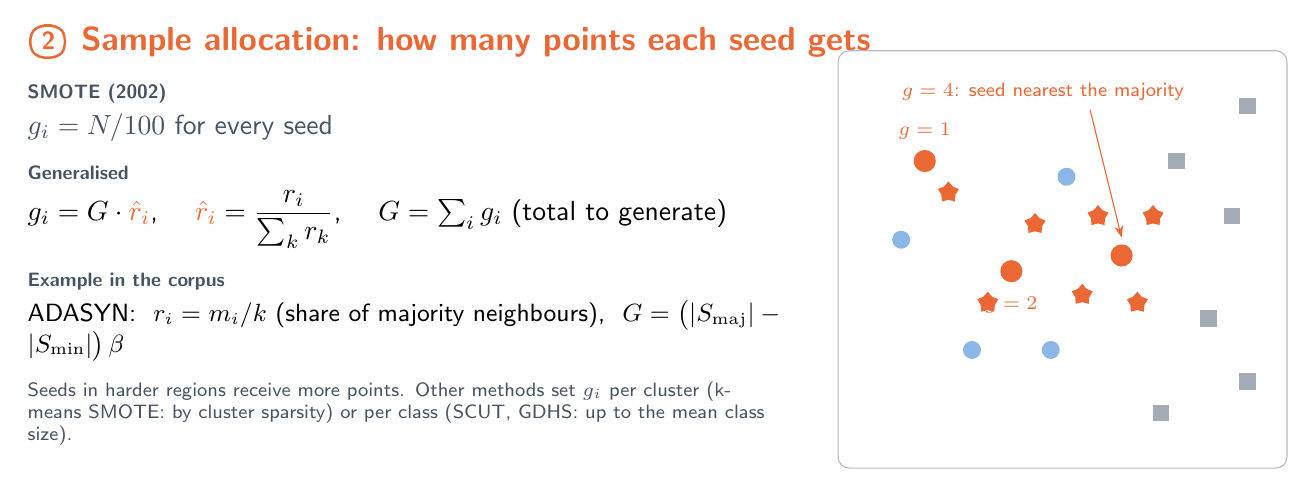
\begin{tikzpicture}
\leftcol{cAlloc}{\textcircled{\small 2} Sample allocation: how many points each seed gets}
 {$g_i = N/100$ for every seed}
 {$g_i = G\cdot \textcolor{cAlloc}{\hat r_i}$, \quad $\textcolor{cAlloc}{\hat r_i} = \dfrac{r_i}{\sum_{k} r_k}$, \quad $G=\textstyle\sum_i g_i$ (total to generate)}
 {ADASYN: \ $r_i = m_i/k$ (share of majority neighbours), \ $G = \bigl(|S_{\mathrm{maj}}|-|S_{\min}|\bigr)\,\beta$}
 {Seeds in harder regions receive more points. Other methods set $g_i$ per cluster (k-means SMOTE: by cluster sparsity) or per class (SCUT, GDHS: up to the mean class size).}
\begin{scope}[shift={(10.6,-5.3)}]
\draw[panel] (-0.3,-0.3) rectangle (5.4,5.0);
\foreach \p in {(4.0,3.6),(4.7,2.9),(4.4,1.6),(4.9,0.8),(3.8,0.4),(4.9,4.3)} \node[mj] at \p {};
\node[circle,fill=cAlloc,minimum size=8pt,inner sep=0pt] (a) at (0.8,3.6) {};
\node[circle,fill=cAlloc,minimum size=8pt,inner sep=0pt] (b) at (1.9,2.2) {};
\node[circle,fill=cAlloc,minimum size=8pt,inner sep=0pt] (c) at (3.3,2.4) {};
\foreach \p in {(0.5,2.6),(1.4,1.2),(2.6,3.4),(2.4,1.2)} \node[mn] at \p {};
\node[sy=cAlloc] at (1.1,3.2) {};
\node[sy=cAlloc] at (1.6,1.8) {}; \node[sy=cAlloc] at (2.2,2.8) {};
\foreach \p in {(3.0,2.9),(2.8,1.9),(3.5,1.8),(3.7,2.9)} \node[sy=cAlloc] at \p {};
\node[font=\scriptsize,text=cAlloc,anchor=south] at (a.north) {$g=1$};
\node[font=\scriptsize,text=cAlloc,anchor=north] at ($(b.south)+(0,-0.05)$) {$g=2$};
\node[font=\scriptsize,text=cAlloc,anchor=south] (cl) at (2.3,4.25) {$g=4$: seed nearest the majority};
\draw[cAlloc,-{Stealth[length=1.5mm]}] (cl.south) ++(0.6,0) -- ($(c.north)+(0,0.08)$);
\end{scope}
\end{tikzpicture}

%% ---------------- 3. neighbour choice ----------------
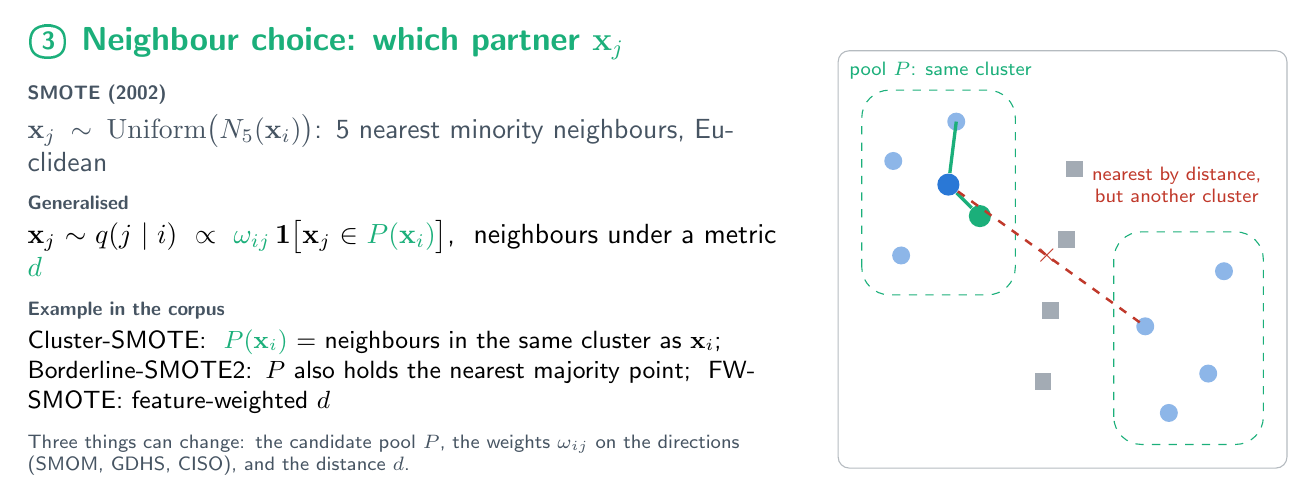
\begin{tikzpicture}
\leftcol{cNbr}{\textcircled{\small 3} Neighbour choice: which partner $\x_j$}
 {$\x_j \sim \mathrm{Uniform}\bigl(N_5(\x_i)\bigr)$: 5 nearest minority neighbours, Euclidean}
 {$\x_j \sim q(j\mid i) \;\propto\; \textcolor{cNbr}{\omega_{ij}}\,\ind\bigl[\x_j\in \textcolor{cNbr}{P(\x_i)}\bigr]$, \ neighbours under a metric $\textcolor{cNbr}{d}$}
 {Cluster-SMOTE: \ $\textcolor{cNbr}{P(\x_i)}$ = neighbours in the same cluster as $\x_i$; \ Borderline-SMOTE2: $P$ also holds the nearest majority point; \ FW-SMOTE: feature-weighted $d$}
 {Three things can change: the candidate pool $P$, the weights $\omega_{ij}$ on the directions (SMOM, GDHS, CISO), and the distance $d$.}
\begin{scope}[shift={(10.6,-5.3)}]
\draw[panel] (-0.3,-0.3) rectangle (5.4,5.0);
\foreach \p in {(2.6,2.6),(2.4,1.7),(2.7,3.5),(2.3,0.8)} \node[mj] at \p {};
\foreach \p in {(0.4,3.6),(1.2,4.1),(0.5,2.4),(1.5,2.9)} \node[mn] at \p {};
\foreach \p in {(3.6,1.5),(4.4,0.9),(4.6,2.2),(3.9,0.4)} \node[mn] at \p {};
\draw[cNbr,dashed,rounded corners=10pt] (0.0,1.9) rectangle (1.95,4.5);
\draw[cNbr,dashed,rounded corners=10pt] (3.2,0.0) rectangle (5.1,2.7);
\node[circle,fill=cSeed,minimum size=8pt,inner sep=0pt] (s) at (1.1,3.3) {};
\node[circle,fill=cNbr,minimum size=8pt,inner sep=0pt] (p) at (1.5,2.9) {};
\draw[cNbr,line width=1.2pt] (s) -- (1.2,4.1);
\draw[cNbr,line width=1.2pt] (s) -- (p);
\draw[cFilt,dashed,line width=0.9pt] (s) -- (3.6,1.5);
\node[cFilt,font=\bfseries] at (2.35,2.4) {$\times$};
\node[font=\scriptsize,text=cNbr,align=center] at (1.0,4.75) {pool $P$: same cluster};
\node[font=\scriptsize,text=cFilt,align=center] at (4.0,3.3) {nearest by distance,\\ but another cluster};
\end{scope}
\end{tikzpicture}

%% ---------------- 4. placement rule ----------------
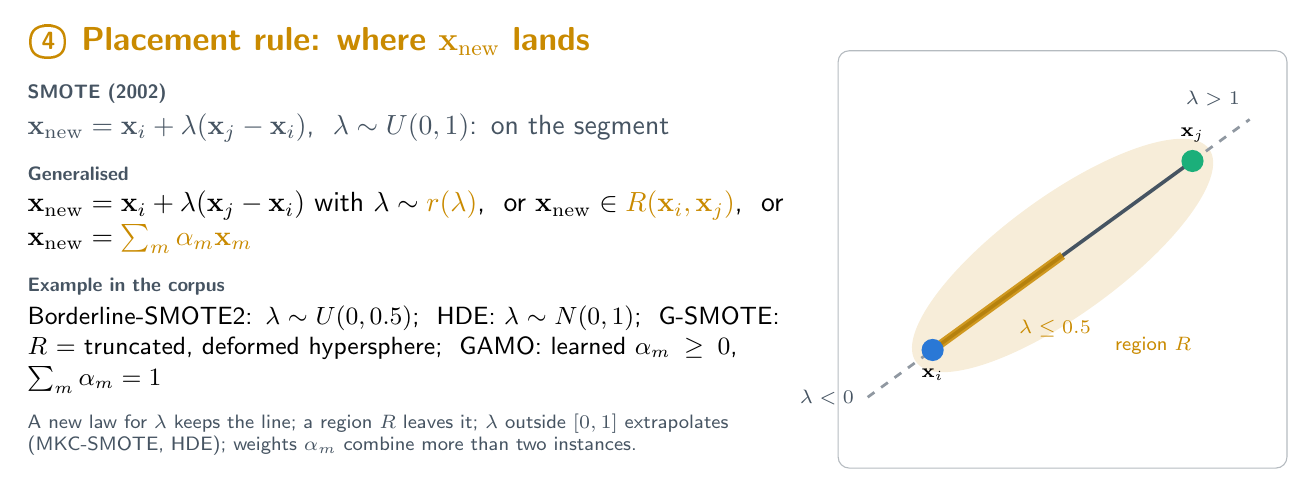
\begin{tikzpicture}
\leftcol{cPlace}{\textcircled{\small 4} Placement rule: where $\x_{\mathrm{new}}$ lands}
 {$\x_{\mathrm{new}} = \x_i + \lambda(\x_j-\x_i)$, \ $\lambda\sim U(0,1)$: on the segment}
 {$\x_{\mathrm{new}} = \x_i + \lambda(\x_j-\x_i)$ with $\lambda\sim \textcolor{cPlace}{r(\lambda)}$, \ or $\x_{\mathrm{new}}\in \textcolor{cPlace}{R(\x_i,\x_j)}$, \ or $\x_{\mathrm{new}}=\textcolor{cPlace}{\sum_m\alpha_m\x_m}$}
 {Borderline-SMOTE2: $\lambda\sim U(0,0.5)$; \ HDE: $\lambda\sim N(0,1)$; \ G-SMOTE: $R$ = truncated, deformed hypersphere; \ GAMO: learned $\alpha_m\ge 0$, $\sum_m\alpha_m=1$}
 {A new law for $\lambda$ keeps the line; a region $R$ leaves it; $\lambda$ outside $[0,1]$ extrapolates (MKC-SMOTE, HDE); weights $\alpha_m$ combine more than two instances.}
\begin{scope}[shift={(10.6,-5.3)}]
\draw[panel] (-0.3,-0.3) rectangle (5.4,5.0);
\coordinate (s) at (0.9,1.2); \coordinate (p) at (4.2,3.6);
\begin{scope}[on background layer]
\fill[cPlace!15,rotate around={36:($(s)!0.5!(p)$)}] ($(s)!0.5!(p)$) ellipse (2.3 and 0.75);
\end{scope}
\draw[inkTwo!60,line width=1pt,dashed] ($(s)!-0.25!(p)$) -- (s);
\draw[inkTwo!60,line width=1pt,dashed] (p) -- ($(s)!1.22!(p)$);
\draw[inkTwo,line width=1.3pt] (s) -- (p);
\draw[cPlace,line width=3pt,opacity=0.85] (s) -- ($(s)!0.5!(p)$);
\node[circle,fill=cSeed,minimum size=8pt,inner sep=0pt] at (s) {};
\node[circle,fill=cNbr,minimum size=8pt,inner sep=0pt] at (p) {};
\node[font=\scriptsize,anchor=north] at ($(s)+(0,-0.12)$) {$\x_i$};
\node[font=\scriptsize,anchor=south] at ($(p)+(0,0.12)$) {$\x_j$};
\node[font=\scriptsize,text=cPlace,anchor=north west] at ($(s)!0.25!(p)+(0.15,-0.1)$) {$\lambda\le 0.5$};
\node[font=\scriptsize,text=cPlace] at (3.7,1.25) {region $R$};
\node[font=\scriptsize,text=inkTwo,anchor=east] at ($(s)!-0.25!(p)+(-0.05,0)$) {$\lambda<0$};
\node[font=\scriptsize,text=inkTwo,anchor=south east] at ($(s)!1.22!(p)+(0,0.05)$) {$\lambda>1$};
\end{scope}
\end{tikzpicture}

%% ---------------- 5. post-filtering ----------------
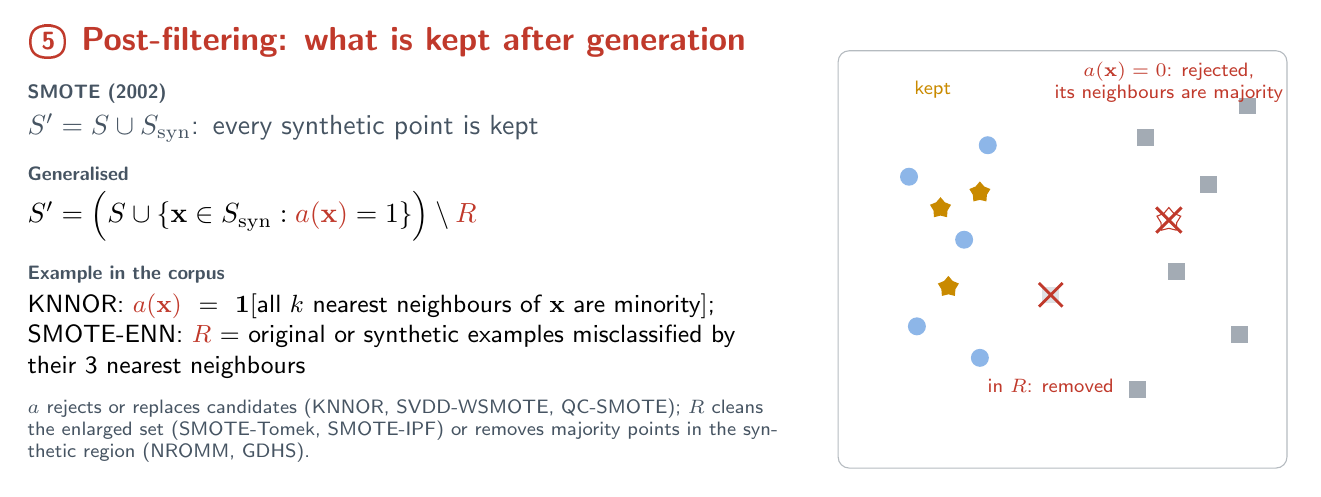
\begin{tikzpicture}
\leftcol{cFilt}{\textcircled{\small 5} Post-filtering: what is kept after generation}
 {$S' = S \cup S_{\mathrm{syn}}$: every synthetic point is kept}
 {$S' = \Bigl(S \cup \{\x\in S_{\mathrm{syn}} : \textcolor{cFilt}{a(\x)}=1\}\Bigr) \setminus \textcolor{cFilt}{R}$}
 {KNNOR: $\textcolor{cFilt}{a(\x)} = \ind[\text{all } k \text{ nearest neighbours of } \x \text{ are minority}]$; \ SMOTE-ENN: $\textcolor{cFilt}{R}$ = original or synthetic examples misclassified by their 3 nearest neighbours}
 {$a$ rejects or replaces candidates (KNNOR, SVDD-WSMOTE, QC-SMOTE); $R$ cleans the enlarged set (SMOTE-Tomek, SMOTE-IPF) or removes majority points in the synthetic region (NROMM, GDHS).}
\begin{scope}[shift={(10.6,-5.3)}]
\draw[panel] (-0.3,-0.3) rectangle (5.4,5.0);
\foreach \p in {(3.6,3.9),(4.4,3.3),(4.0,2.2),(4.8,1.4),(3.5,0.7),(4.9,4.3)} \node[mj] at \p {};
\node[mj,opacity=0.35] (rm) at (2.4,1.9) {};
\draw[cFilt,line width=1pt] ($(rm)+(-0.15,-0.15)$)--($(rm)+(0.15,0.15)$) ($(rm)+(-0.15,0.15)$)--($(rm)+(0.15,-0.15)$);
\foreach \p in {(0.6,3.4),(1.3,2.6),(0.7,1.5),(1.6,3.8),(1.5,1.1)} \node[mn] at \p {};
\foreach \p in {(1.0,3.0),(1.1,2.0),(1.5,3.2)} \node[sy=cPlace] at \p {};
\node[star,star points=5,draw=cFilt,fill=white,minimum size=9pt,inner sep=0pt] (bad) at (3.9,2.85) {};
\draw[cFilt,line width=1.1pt] ($(bad)+(-0.16,-0.16)$)--($(bad)+(0.16,0.16)$) ($(bad)+(-0.16,0.16)$)--($(bad)+(0.16,-0.16)$);
\node[font=\scriptsize,text=cFilt,align=center] at (3.9,4.6) {$a(\x)=0$: rejected,\\ its neighbours are majority};
\node[font=\scriptsize,text=cFilt,align=center] at (2.4,0.75) {in $R$: removed};
\node[font=\scriptsize,text=cPlace] at (0.9,4.5) {kept};
\end{scope}
\end{tikzpicture}

%% ---------------- 6. inside a pipeline ----------------
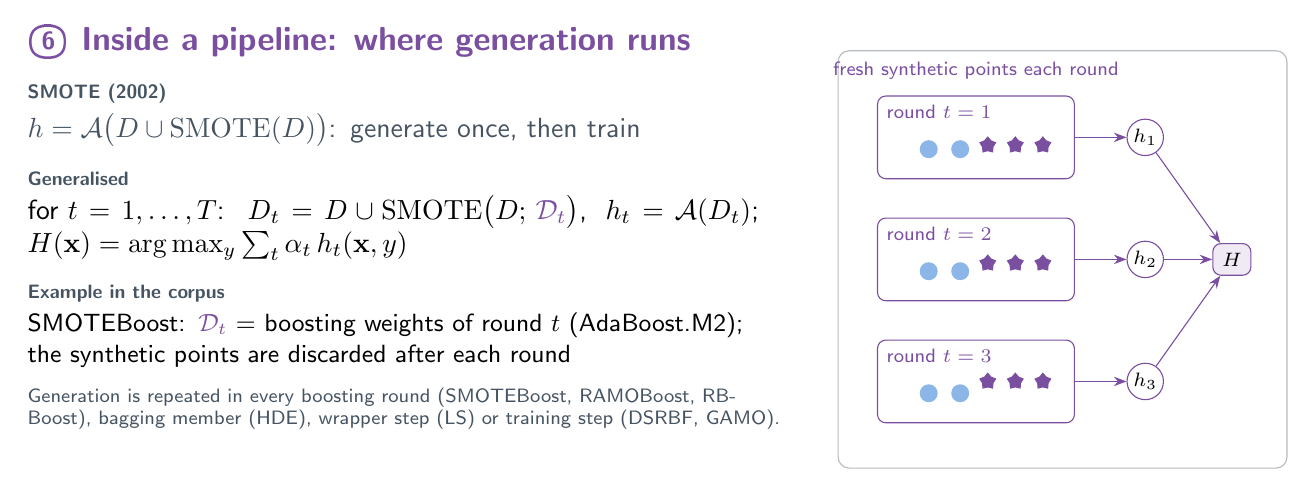
\begin{tikzpicture}
\leftcol{cPipe}{\textcircled{\small 6} Inside a pipeline: where generation runs}
 {$h = \mathcal{A}\bigl(D \cup \mathrm{SMOTE}(D)\bigr)$: generate once, then train}
 {for $t=1,\dots,T$: \ $D_t = D \cup \mathrm{SMOTE}\bigl(D;\,\textcolor{cPipe}{\mathcal{D}_t}\bigr)$, \ $h_t=\mathcal{A}(D_t)$; \quad $H(\x)=\arg\max_y \sum_t \alpha_t\, h_t(\x,y)$}
 {SMOTEBoost: $\textcolor{cPipe}{\mathcal{D}_t}$ = boosting weights of round $t$ (AdaBoost.M2); the synthetic points are discarded after each round}
 {Generation is repeated in every boosting round (SMOTEBoost, RAMOBoost, RBBoost), bagging member (HDE), wrapper step (LS) or training step (DSRBF, GAMO).}
\begin{scope}[shift={(10.6,-5.3)}]
\draw[panel] (-0.3,-0.3) rectangle (5.4,5.0);
\foreach \t/\y in {1/3.9,2/2.35,3/0.8} {
  \node[draw=cPipe,rounded corners=3pt,minimum width=2.5cm,minimum height=1.05cm] (r\t) at (1.45,\y) {};
  \node[font=\scriptsize,text=cPipe,anchor=north west] at (r\t.north west) {round $t=\t$};
  \foreach \dx in {0.35,0.75} \node[mn] at ($(r\t.center)+(\dx-0.95,-0.15)$) {};
  \foreach \dx in {0.15,0.5,0.85} \node[sy=cPipe,minimum size=6.5pt] at ($(r\t.center)+(\dx,-0.15+0.05*\t)$) {};
  \node[draw=cPipe,circle,inner sep=1pt,font=\scriptsize] (h\t) at (3.6,\y) {$h_{\t}$};
  \draw[-{Stealth[length=1.6mm]},cPipe] (r\t) -- (h\t);
}
\node[draw=cPipe,fill=cPipe!12,rounded corners=3pt,font=\scriptsize] (H) at (4.7,2.35) {$H$};
\foreach \t in {1,2,3} \draw[-{Stealth[length=1.6mm]},cPipe] (h\t) -- (H);
\node[font=\scriptsize,text=cPipe] at (1.45,4.75) {fresh synthetic points each round};
\end{scope}
\end{tikzpicture}

\end{document}
